\documentclass{book}

\usepackage{hyphenat} % http://www.ctex.org/documents/packages/special/hyphenat.pdf

\usepackage{setspace}\onehalfspacing\frenchspacing\flushbottom\sloppy

\usepackage{hyperref}
\hypersetup{
    colorlinks=true,
    linkcolor=blue,
    filecolor=magenta,      
    urlcolor=cyan,
    pdftitle={Overleaf Example},
    pdfpagemode=FullScreen,
    }

% https://en.wikibooks.org/wiki/LaTeX/Glossary says
% "\usepackage{glossaries} and \makeglossaries in your preamble (after \usepackage{hyperref} if present)"

% https://www.overleaf.com/learn/latex/Glossaries
\usepackage[toc]{glossaries}

\makeglossaries % The command must be before the first glossary entry.

% https://en.wikibooks.org/wiki/LaTeX/Glossary says
% "define any number of \newglossaryentry and \newacronym glossary and acronym entries in your preamble"
% see https://en.wikibooks.org/wiki/LaTeX/Glossary
% and https://www.overleaf.com/learn/latex/Glossaries

\newglossaryentry{organization}{
  name={organization},
  plural={organizations},
  description={an assembly of teams. The name of the concept might be a corporation, an agency, a department, a bureau, or any other aggregation of smaller organizations}
}

\newglossaryentry{culture}{
name={culture},
plural={cultures},
description={norms, expectations around interaction among people}
}

\newglossaryentry{stakeholder}{
name={stakeholder},
plural={stakeholders},
description={a person who cares about the process or the outcome; distinct from a participant}
%descriptionplural={people who cares about the process or the outcome; distinct from participants}
}

\newglossaryentry{participant}{
name={participant},
description={a person who is expected to take action or make contribution}
}

\newglossaryentry{essential bureaucracy}{
name={essential bureaucracy},
text={Essential bureaucracy},
description={the minimum processes and staffing and skills necessary to address the complexity of the problem space}
}

\newglossaryentry{bureaucratic debt}{
name={bureaucratic debt},
plural={bureaucratic debts},
text={Bureaucratic debt},
description={the cost of work need to change a process caused by choosing an easy solution now instead of using a better approach that would take longer}
}

\newglossaryentry{subject}{
    name={subject},
    plural={subjects},
    description={the person experiencing bureaucracy}
}
\newglossaryentry{Prisoner's dilemma}{
    name={Prisoner's dilemma},
    description={Two or more people with incomplete information of a situation will make suboptimal choices compared to someone with perfect knowledge of the situation}
}

\newglossaryentry{thought terminating}{
name={thought terminating},
description={\href{https://en.wikipedia.org/wiki/Thought-terminating_clich\%C3\%A9}{thought terminating statements} initially sound reasonable but, upon reflection and analysis, are incorrect}
}

\newglossaryentry{presence creates priority}{
name={presence creates priority},
description={being physically at a person's desk motivates that person to respond better than calling them or emailing them}
}

% https://graphthinking.blogspot.com/2021/07/bureaucracy-book-outline.html
\newglossaryentry{bureaucrat}{
    name={bureaucrat},
    plural={bureaucrats},
    description={the person who is a member of an organization and is responsible for subjective implementation of policy for the organization. Conventional examples of a bureaucrat role: teacher, police, government employee}
}

\newglossaryentry{simple decision}{
  name={simple decision},
  description={has one correct or beneficial choice and one or more wrong or harmful choices.}
}

% https://tex.stackexchange.com/questions/69567/uppercase-word-in-glossary-lowercase-in-text
\newglossaryentry{bureaucracy}{
    name={bureaucracy},
    plural={bureaucracies},
    text={bureaucracy},
    description={
    An organization of bureaucrats comprises a bureaucracy. A bureaucracy facilitates coordination of stakeholders. 
    Bureaucracy is how large organizations make distributed decisions using distributed knowledge.    \\
    Everything in a bureaucracy is made up by other participants. \\
    Bureaucracy is a macroscopic phenomenon emergent at sufficient scale. The scale is important because there is no longer dependence on individual relationships. \\
    Bureaucracy arises when there is no common objectively quantifiable feedback mechanism for individual participants in the organization.\\
    Bureaucracy is a wicked problem}
}

\newglossaryentry{visible bureaucracy}{
name={visible bureaucracy},
    %name={bureaucracy, visible},
    description={procedures and processes are written down and can be discovered by stakeholders}
}
\newglossaryentry{invisible bureaucracy}{
name={invisible bureaucracy},
    %name={bureaucracy, invisible},
    description={procedures and processes are known to some stakeholders and are conveyed verbally to some of the other stakeholders}
}

\newglossaryentry{process}{
name={process},
plural={processes},
description={a task broken into a specified set of subtask dependencies}
}



\title{Bureaucracy Guidebook: How to be an effective bureaucrat}
\author{Ben Payne}
\date{\today}

\begin{document}

\maketitle
\frontmatter % the front of the book has roman numerals

\thispagestyle{empty}

Copyright \copyright 2022 Ben Payne

\ \\

\href{https://creativecommons.org/licenses/by-nc/4.0/}{Creative Commons Attribution-NonCommercial 4.0 International License}
%\clearpage

\thispagestyle{empty}

Thank you to my coworkers. Our interactions me learn how to be a better bureaucrat.%\clearpage

\chapter*{Foreword}% * excludes from Contents)

% Who this book is for

%If you don't think of yourself as a bureaucrat, I hope to change your mind on this essential topic. 
If you have a negative impression of bureaucracy, I want to convince you that bureaucracy is vital and that you can learn to skillfully navigate bureaucracy.

I see this struggle of bureaucracy as critical to modern society. The challenge of bureaucracy is widespread across a variety of governments in different societies, and bureaucracy is durable -- it has existed for hundreds if not thousands of years. Therefore, tackling the challenge of bureaucracy is exciting for me. I enjoy pondering hard problems and then leveraging insights gained from reflection. Being an effective bureaucrat is important to me because bureaucracy can be a force multiplier beyond what I could accomplish on my own.

% from https://graphthinking.blogspot.com/2021/07/bureaucracy-book-outline.html
This book is for you if you are curious about the complex world we live in, or you are thinking about how to productively contribute to society, or you want impactful employment, or your job is not what you expected. If you're wondering why innovation is hard within a bureaucratic organization, this guidebook is intended to help understand what the challenges are.


% What you should expect reading this book: 
Everyone in modern society is a participant in bureaucracy. The purpose of this book is to decrease the surprise of that experience and better arm you emotionally and intellectually for the toil of being a bureaucrat. With focused reflection and a good guidebook, you can improve your skills as a bureaucrat. 

This book is neither a defense of bureaucracy, nor is it intended to disparage bureaucrats or the system of bureaucracy. Instead, the intent of this book is to serve as a guide to bureaucracy-as-it-is. 

This book does not focus on leadership, managing a team, being a team member, planning, time management, project management, advancing your career, or self-improvement. However, in the process of being a better bureaucrat some lessons may apply in those domains.

This book doesn't address personal stress caused by bureaucracy, how to decrease stress, or how to balance the activities of work and life-outside-work. 

This book doesn't focus on citizens, Congress (state or federal), or competing organizations. 

This book doesn't address discrimination or harassment. This book doesn't address bad coworkers, abusive bosses, psychological defects of individuals, or malicious intent. Issues like lying, bribery, and criminal behavior are not discussed. All these aspects happen whenever people interact; the challenges are not specific to bureaucracy. In this book I assume you are honest, and that other people are honest. Even with this simplifying assumption the complexities of bureaucracy arise. In the context of that benign bureaucracy, guidance on how to be an effective bureaucrat is provided.


% What is the benefit of reading this book?
As a result of reading this book, you will be better able to recognize and navigate complex professional environments, both within your career and outside of work. The perspectives offered in this book can benefit you directly, whether by promotion of title, increase in pay, successful completion of a project, or through decreased stress of understanding how the world operates. Being a more effective bureaucrat can also positive impact the causes you care about and the people you engage with.

If you do not recognize that you are bureaucrat, you won't know what is your own fault, the fault of your coworkers, the fault of management, and what is intrinsic to bureaucracy. 

If you do not recognize that you are bureaucrat, you're less likely to be successful interacting with those around you. The self-recognition of being a bureaucrat matters; how you behave and what you think your responsibilities are depend on how you label yourself.

Even people who are smart (e.g., they know history, they have memorized capital cities, they can do math) can struggle in the face of complex large-scale systems. Thinking about complex large-scale systems is not part of the education curriculum. This book will help you learn about bureaucracy and lead to an increase of your ability to identify patterns and apply relevant techniques.

% there's no avoiding the issue
Everyone is a bureaucrat because there are no alternatives to bureaucracy for a society. Gaining skills in navigating bureaucracy are helpful both for your own happiness and the well-being of a functioning society. 

Hoping that modern technology will eliminate or reduce bureaucracy is not helpful. Automation and computers merely obfuscate processes and make negotiation more challenging. 

Simplifying interactions with other people to ``this is characterized merely as human relations" is an easier perspective compared to considering bureaucracy as a complex system. 
% this is also stated on page 24 of \cite{1991_Wilson}
However, a simplified view either misses emergent phenomena or mischaracterizes the situation. In either case, your effectiveness is harmed.



% my experience
% I wrote this book for a younger version of me.
 When I first started my job in a large organization I recognized differences between the expectations of the education system I had left and the challenges of a professional environment. Over the years I learned from my mistakes by reflecting on my (in)actions and the consequences. This approach has been an expensive education. My mistakes delayed progress and damaged relationships. The motive in this book is to provide generalizations from my experiences which might benefit the reader.


% Caveats

In my reflections and attempting to draw lessons there is a risk of overanalysis. Sometimes a situation is merely happenstance, and sometimes attempting to extract lessons from randomness is folly. Avoiding conjecture about conspiracy and malice is a fuzzy boundary when insufficient information is available. 

My experiences cannot be generalized to every situation. Some of the observations here may be analogous to your context if you squint. 

Nothing in this book is domain specific, nothing is tied to engineering of products, and nothing is applicable solely in science research or policy development. While this material is intended to be timeless and generic, it is culturally specific to the United States of America in the early twenty first century. There are cultural blindspots not addressed in this book because I did not encounter systemic hurdles in my career as financially privileged white male. 

% Source of this content: 
This material is based on personal experience, reading published materials, and anecdotes from other people. No surveys were taken to support the claims made. No double blind experiments were conducted. 

% How the book should be read: 
Reading this book front-to-back is the default option. 
%Chapter~\ref{b_throughout_life} provides context for the lifelong experience of bureaucracy. 
The essentials of bureaucracy described in \S~\ref{fundamentals_of_b} will be familiar to experienced bureaucrats. Each section in Chapter~\ref{b_made_of_humans} is intended to be able to be read stand-alone. The content is intended to spark contemplation. 

\ \\

% as per https://tex.stackexchange.com/q/393238/235813
\begin{flushright}
Ben Payne\\
\today\\
United States of America\\
Earth
\end{flushright}


%\clearpage


\tableofcontents

\mainmatter % the main part of the book will have standard pages



\chapter{Introduction to Bureaucracy}
% essentials

\section{Fundamentals of Bureaucracy}

\subsection{What is bureaucracy?}
While you may know it when you see it or experience it, for this book a definition is useful. 
\gls{bureaucracy} is coordination of stakeholders. This concept is most visible for complex, long lasting, and recurring situations involving many people. The apparent friction can be lower when there are only a few people involved ("I'm just talking to my collaborator"), but there is a continuous gradient. 


\subsection{Why does bureaucracy exist? Can't we just do the work?}

The minimal scenario to start from is to imagine a single person working on a single task that does not last long (a few minutes), is relatively easy (cognitively and physically and emotionally), and does not recur. Most of what you do occurs outside those limits and thus incurs some concept of \gls{process} (breaking a task into subtasks). Staying with the one-person constraint, a complex task can benefit from being broken into subtasks where order of the subtasks matters. 

% https://graphthinking.blogspot.com/2021/09/why-is-everything-so-hard-in-large.html



\subsection{Hierarchy of roles}

\subsection{Org chart as a guide and a lie}

lie in the sense that undocumented relationships matter more than the roles

lie in the sense of orientation; see \ref{org-chart-orientation}

\subsection{Approval process}

\subsection{Meetings for coordination}

coordination and signaling

\subsection{Written communication}

Reports, memos, emails are artifacts of bureaucracy. They create evidence and can be used for good or bad. 



\chapter{Bureaucracies are made of Humans}
% unordered essays to be clustered latter

\subsubsection{Organization chart orientation
\label{org-chart-orientation}}

A common method of describing relations within the bureaucracy is the organization chart (colloquially, the ``org chart"). Normally the CEO is at the top of the chart, middle management is in the middle, and managed employees are at the bottom. See figure~\ref{org_chart_orientation_ceo-at-top} 


An organization's culture is subtly conveyed by artifacts like org charts. 
% What's the point of this section? Is there a consequence, or is this just an observation?
There are emotional connotations to alternative layouts. You can alter expected relations (culture and norms) by playing with orientation of the org chart.
Org chart orientation can be overanalyzed, so this exploration is limited.

The point of thinking about org chart orientation is to frame how you perceive your supervisors, peers, subordinates. Notice that the framing is embedded in the words -- prefixes super (over) and sub (under). 
These concepts inform what you expect from relations.
Do I seek support or direction and guidance from my boss? What do I expect from my boss, peers subordinates? What do I expect to provide them?

%\begin{itemize}
%\item 
%\end{itemize}

The relative orientation of the \href{https://en.wikipedia.org/wiki/Chief_executive_officer}{CEO} to workers sets expectations for relations. 
Options for orientation are the conventional CEO at top
(figure~\ref{org_chart_orientation_ceo-at-top}), 
CEO at the bottom (figure~\ref{org_chart_orientation_ceo-at-bottom}),
CEO on the right (figure~\ref{org_chart_orientation_ceo-leads}),
CEO on the left (figure~\ref{org_chart_orientation_ceo-follows}),
CEO as the center of a star 
(Example: \href{https://en.wikipedia.org/wiki/File:League_of_Nations_Organization.png}{League of Nations diagram})

\begin{figure}
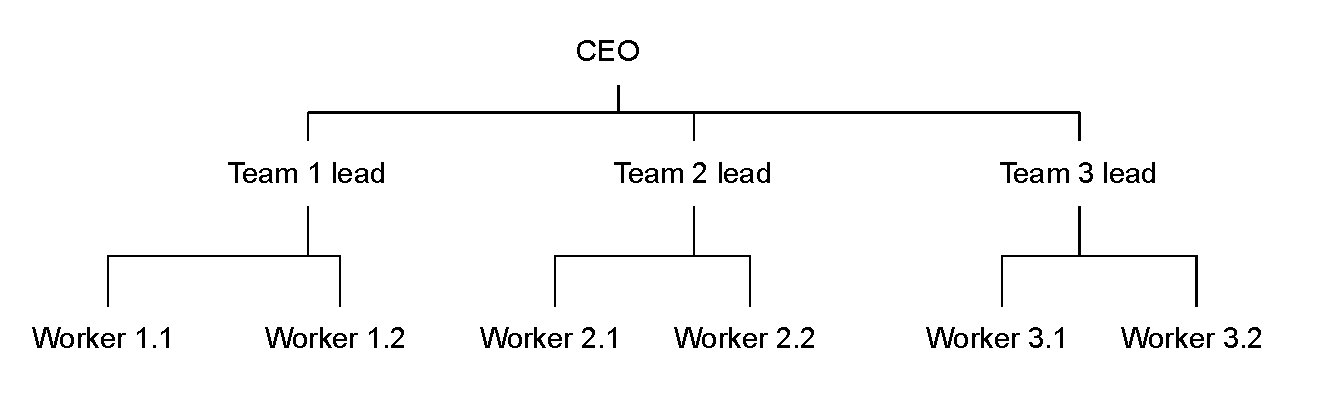
\includegraphics[width=1\textwidth]{images/org-chart-orientation-ceo-at-top.pdf}
\caption{Standard orientation. Role with most responsibility and authority is at top. Left-right ordering is intended to be irrelevant in this view, though left-to-right reading order emphasizes importance.}
\label{org_chart_orientation_ceo-at-top}
\end{figure}

\begin{figure}
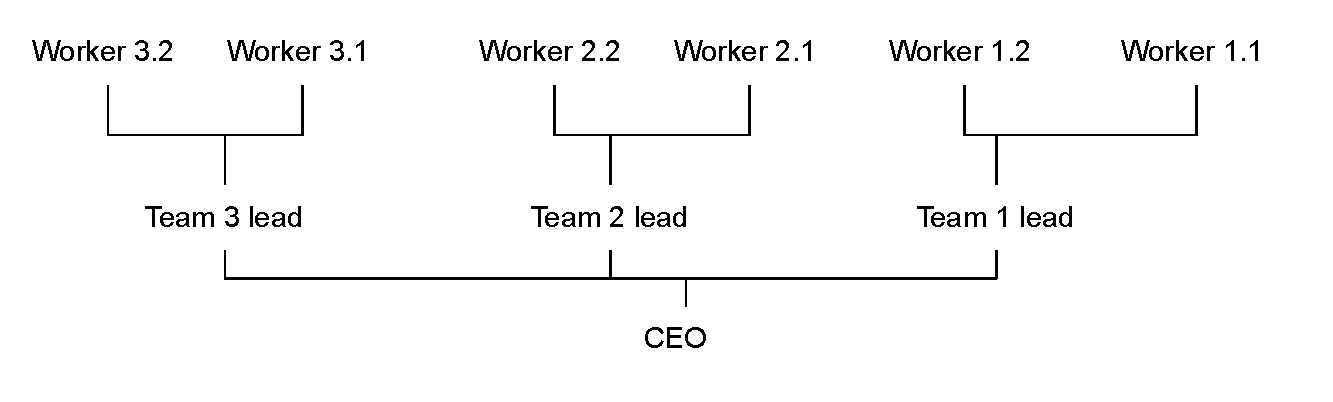
\includegraphics[width=1\textwidth]{images/org-chart-orientation-ceo-at-bottom.pdf}
\caption{Flipping the orientation presents a more realistic view of the CEO's responsibility. The crushing burden of servant leadership is clear. Left-right ordering is intended to be irrelevant in this view.}
\label{org_chart_orientation_ceo-at-bottom}
\end{figure}

\begin{figure}
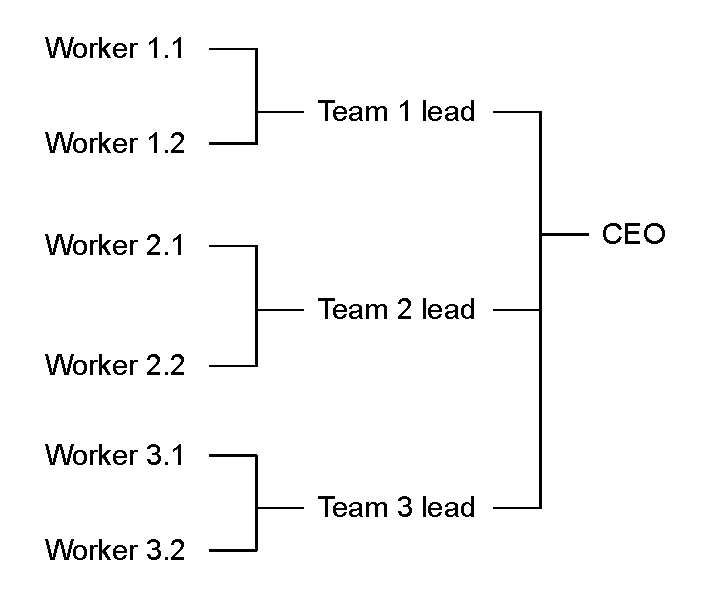
\includegraphics[width=0.8\textwidth]{images/org-chart-orientation-ceo-leads.pdf}
\caption{Conventionally time flows from left (old) to right (new), so in this graph the CEO leads the charge into the unknown. Is the CEO dragging workers forward, or are the workers pushing the CEO? The top-to-bottom ordering can be read as importance. }
\label{org_chart_orientation_ceo-leads}
\end{figure}

\begin{figure}
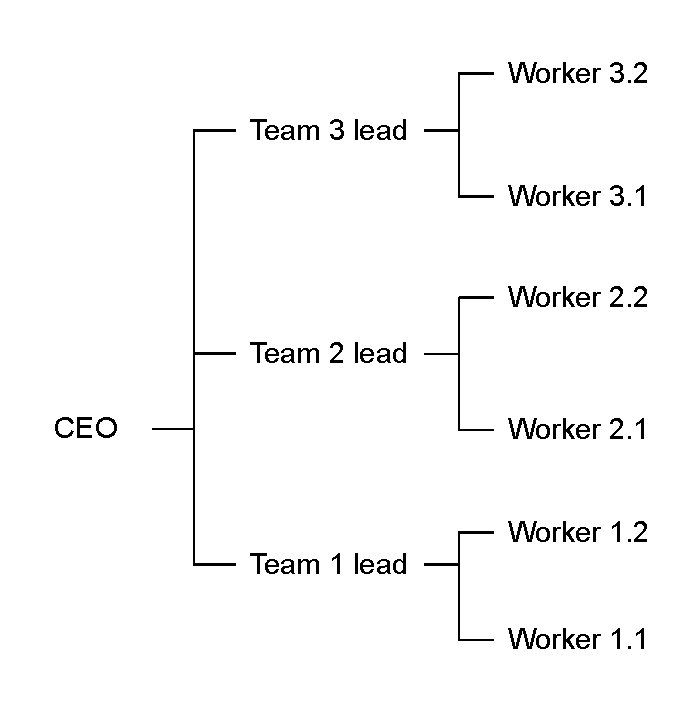
\includegraphics[width=0.8\textwidth]{images/org-chart-orientation-workers-lead.pdf}
\caption{The ``chariot view'' with the CEO in the chariot and the workers out front. Workers are in the future, the CEO is in the past operating on old information. As with figure~\ref{org_chart_orientation_ceo-leads}, top-to-bottom ordering can be read as importance. }
\label{org_chart_orientation_ceo-follows}
\end{figure}



%extension of 
% \href{https://en.wikipedia.org/wiki/Conway\%27s_law}{Conway's law}: seating chart reflects org chart

% https://graphthinking.blogspot.com/2020/05/invisible-bureaucracy.html

\subsection{Social and Bureaucratic interactions}

Interactions with other people in an organization are either social interaction or bureaucratic interaction. 

As examples of each of these,
\begin{itemize}
\item Social interaction example: "Did you see the game on TV last night? Our team really did well, right? I thought about getting tickets for the game but they were sold out."
\item Bureaucratic interaction example: "You'll need to get approval from Sue before presenting your idea to the board for their review. Then talk with Russ and get his thoughts."
\end{itemize}
Both social and bureaucratic interactions are vital to cohesion in an organization of people. 


Bureaucratic interaction can be broken into two subcategories: \gls{visible bureaucracy} (procedures and processes are written down and can be discovered by stakeholders)  and \gls{invisible bureaucracy} (procedures and processes are known to some stakeholders and are conveyed verbally to some of the other stakeholders).

Invisible bureaucracy is akin to invisible domestic or relation work outside the professional environment. The work associated with emotional cohesion, logistics, planning, scheduling, and communicating is hard to quantify so it does not get counted.

To make invisible work and invisible bureaucracy visible, document the work.


The relevance of this jargon is to break down the components of an organization's "culture" experienced by participants. The ratio of social/visible bureaucracy/invisible bureaucracy is a characterization of the culture. There are norms associated with each of these three categories.

% https://graphthinking.blogspot.com/2021/02/how-to-have-efficient-bureaucracy.html

In an ideal scenario with no bureaucracy, everyone comes to the same conclusion when presented with the same information. Then the management process of building consensus becomes unnecessary. There is no need to fight over resources (money, staffing) and no need to fight over direction.

While that ideal scenario is not going to happen, it points to how to improve bureaucratic efficiency:
\begin{itemize}
\item each person has the same information. 
\item each person applies the same decision making process consistently
\item every person has the same incentives
\end{itemize}
The reason bureaucracy is inefficient is
\begin{itemize}
\item not everyone has the same information
\item processes are inconsistent
\item incentives vary
\end{itemize}
Also, add the issue that each person's reference experiences are unique. As a consequence, decision making is subjective. 

Can any action be taken to improve bureaucratic efficiency? Yes!
\begin{itemize}
\item you can share information with other stakeholders
\item you can seek information from other stakeholders
\item you can strive for and demonstrate transparency
\item apply consistent processes 
\item hold others (and yourself) accountable 
\item account for varying incentives and reference experiences
\end{itemize}


% https://graphthinking.blogspot.com/2021/04/laffer-curve-and-minimum-viable.html

The Laffer curve is a claim in economics that there is a relation between government tax rates and the revenue from taxes collected. The relation, based on Rolle's theorem, says that between a tax rate of 0% and 100%, there must be some amount of tax that corresponds to the maximum of revenue. 

While the mathematical statement may be provable, the use in economics seems hand-wavy. In this post, I'll extend that hand-waviness to a different domain: bureaucratic processes in organizations. The relation to the Laffer curve is that bureaucratic processes a tax on productivity. 

\clearpage

\printglossaries

\nocite{*} % causes LaTeX to include every entry in your .bib file.
\bibliographystyle{plain-annote}
\bibliography{biblio}

\end{document}
